\interlude[2]<Trials \textasciitilde\ Attacks found>{ChronoTrigger}
\hypertarget{state-disruption}{%
\section{State Disruption}\label{state-disruption}}




\begin{frame}{What are Non-Interruptability\\and State Disruption Attacks?}
  \begin{itemize}
    \item Attacker trying to perform a protocol-level DOS attack
    \item Attacker may observe messages
    \item Attacker may insert messages, but they may not drop or modify messages
    \item Halfway between an active and passive attacker:
    \begin{itemize}
    \item For a fully active attacker state disruption is trivial; they can just drop messages
    \end{itemize}
  \end{itemize}
\end{frame}




\begin{frame}{Retransmission Protection in WireGuard}
\hypertarget{retransmission-protection-in-wireguard}{}
\begin{columns}[fullwidth,T]
  \begin{column}{.5\linewidth}
  \rlap{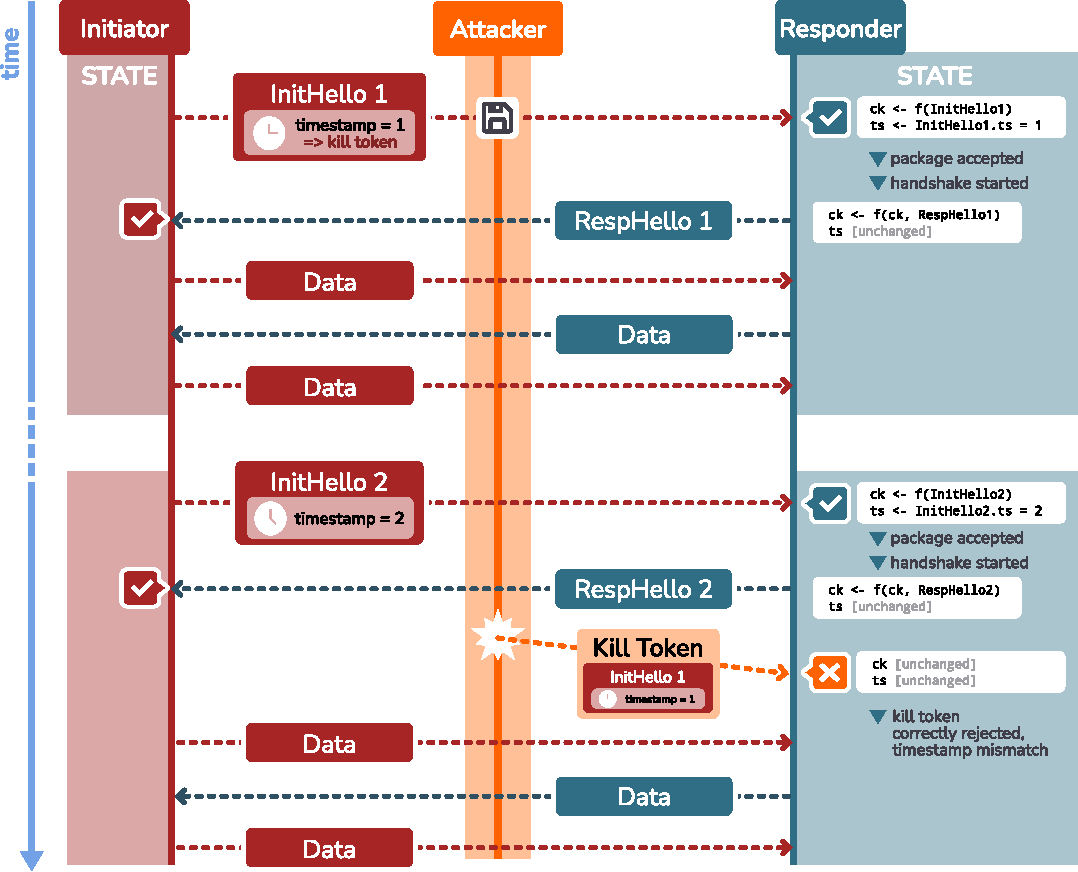
\includegraphics[height=.85\textheight]{graphics/wg-retransmission-protection-bare.pdf}}
  \end{column}
  \begin{column}{.46\linewidth}
  \small
    \begin{itemize}
    \item Replay attacks thwarted by counter
    \item Counter is based on real-time clock
    \item Responder is semi-stateful (one retransmission at program start may be accepted, but this does not affect protocol security)
    \item[$\Rightarrow$]
       WG requires \emph{either} reliable real-time clock \emph{or} stateful initiator
    \item[$\Rightarrow$]
      Adversary can attempt replay, but this cannot interrupt a valid handshake by the initiator
    \item[!] Assumption of reliable system time is invalid in practice!
    \end{itemize}
  \end{column}
\end{columns}
\end{frame}




\begin{frame}{ChronoTrigger Attack}
\begin{columns}[fullwidth,T]
  \begin{column}{.5\linewidth}
          \rlap{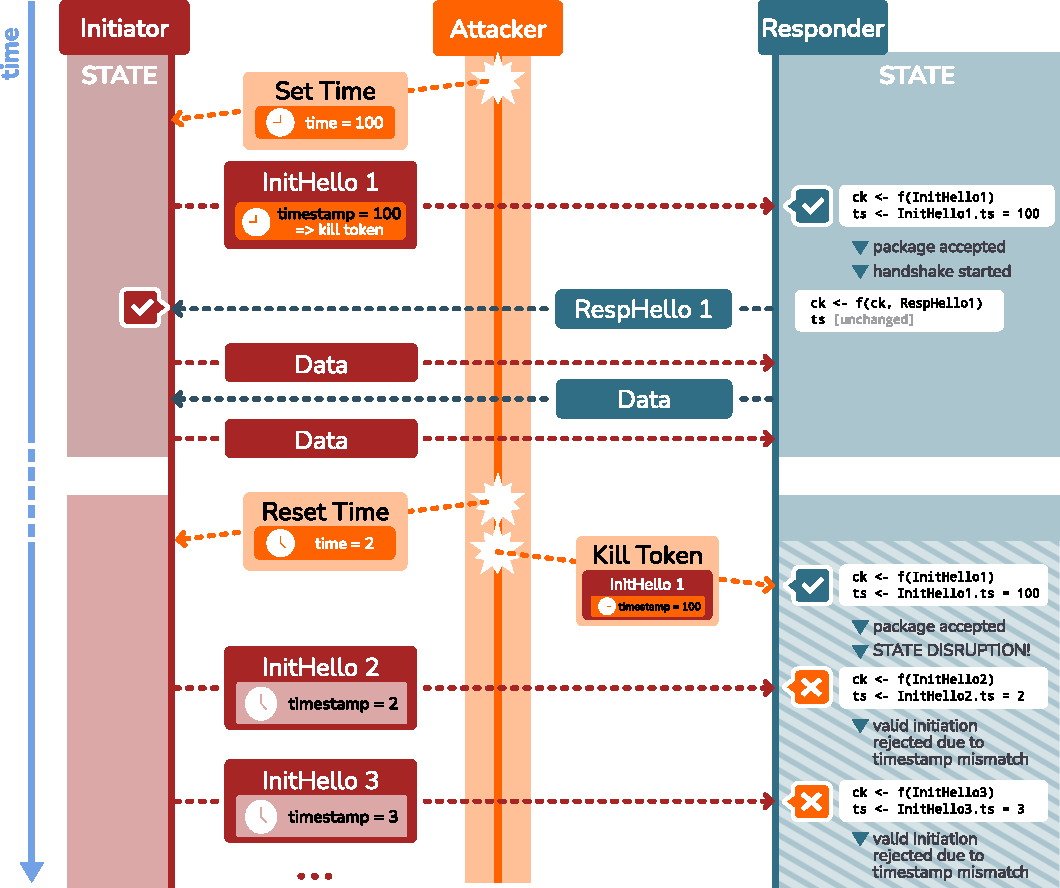
\includegraphics[height=.85\textheight]{graphics/chronotrigger-bare.pdf}}
  \end{column}

  \begin{column}{.46\linewidth}
    \small\leavevmode
    \only<+|handout:+>{
      \begin{enumblock}{Preparation phase:}
      \begin{enumerate}
        \item \textbf{Attacker} sets \emph{initiator system time} to a future value
        \item \textbf{Attacker} records \emph{InitHello} as \emph{KillToken} while both peers are performing a valid handshake
      \end{enumerate}
      \end{enumblock}
\centerline{ \small … both peers are being reset … }
      \begin{enumblock}{Delayed execution phase:}
      \begin{enumerate}
        \item \textbf{Attacker} sends \emph{KillToken} to responder, setting their timestamp to a future value
        \item[$\Rightarrow$] Initiation now fails again due to timestamp mismatch
      \end{enumerate}
      \end{enumblock}
    }

    \only<+|handout:+>{%
      \begin{block}{Gaining access to system time:}
      \begin{itemize}
        \item Network Time Protocol is insecure,\\
        Mitigations are of limited use
        \item[$\Rightarrow$] Break NTP \emph{once}; kill token lasts forever
      \end{itemize}
      \unskip
      \end{block}
    }

    \only<+|handout:+>{%
      \leavevmode\begin{block}{Attacker gains}
      \begin{itemize}
        \item Extremely cheap protocol-level DOS
      \end{itemize}
      \unskip
      \end{block}

      \begin{block}{Preparation phase, attacker needs:}
      \begin{itemize}
        \item Eavesdropping of initiator packets
        \item Access to system time
      \end{itemize}
      \unskip
      \end{block}

      \begin{block}{Delayed execution, attacker needs:}
      \begin{itemize}
        \item No access beyond message transmission to responder
      \end{itemize}
      \unskip
      \end{block}
  }
  \end{column}
\end{columns}
\end{frame}




\begin{frame}{ChronoTrigger: Changes in Rosenpass}
  \begin{columns}[fullwidth,c]
    \begin{column}{.64\linewidth}
      %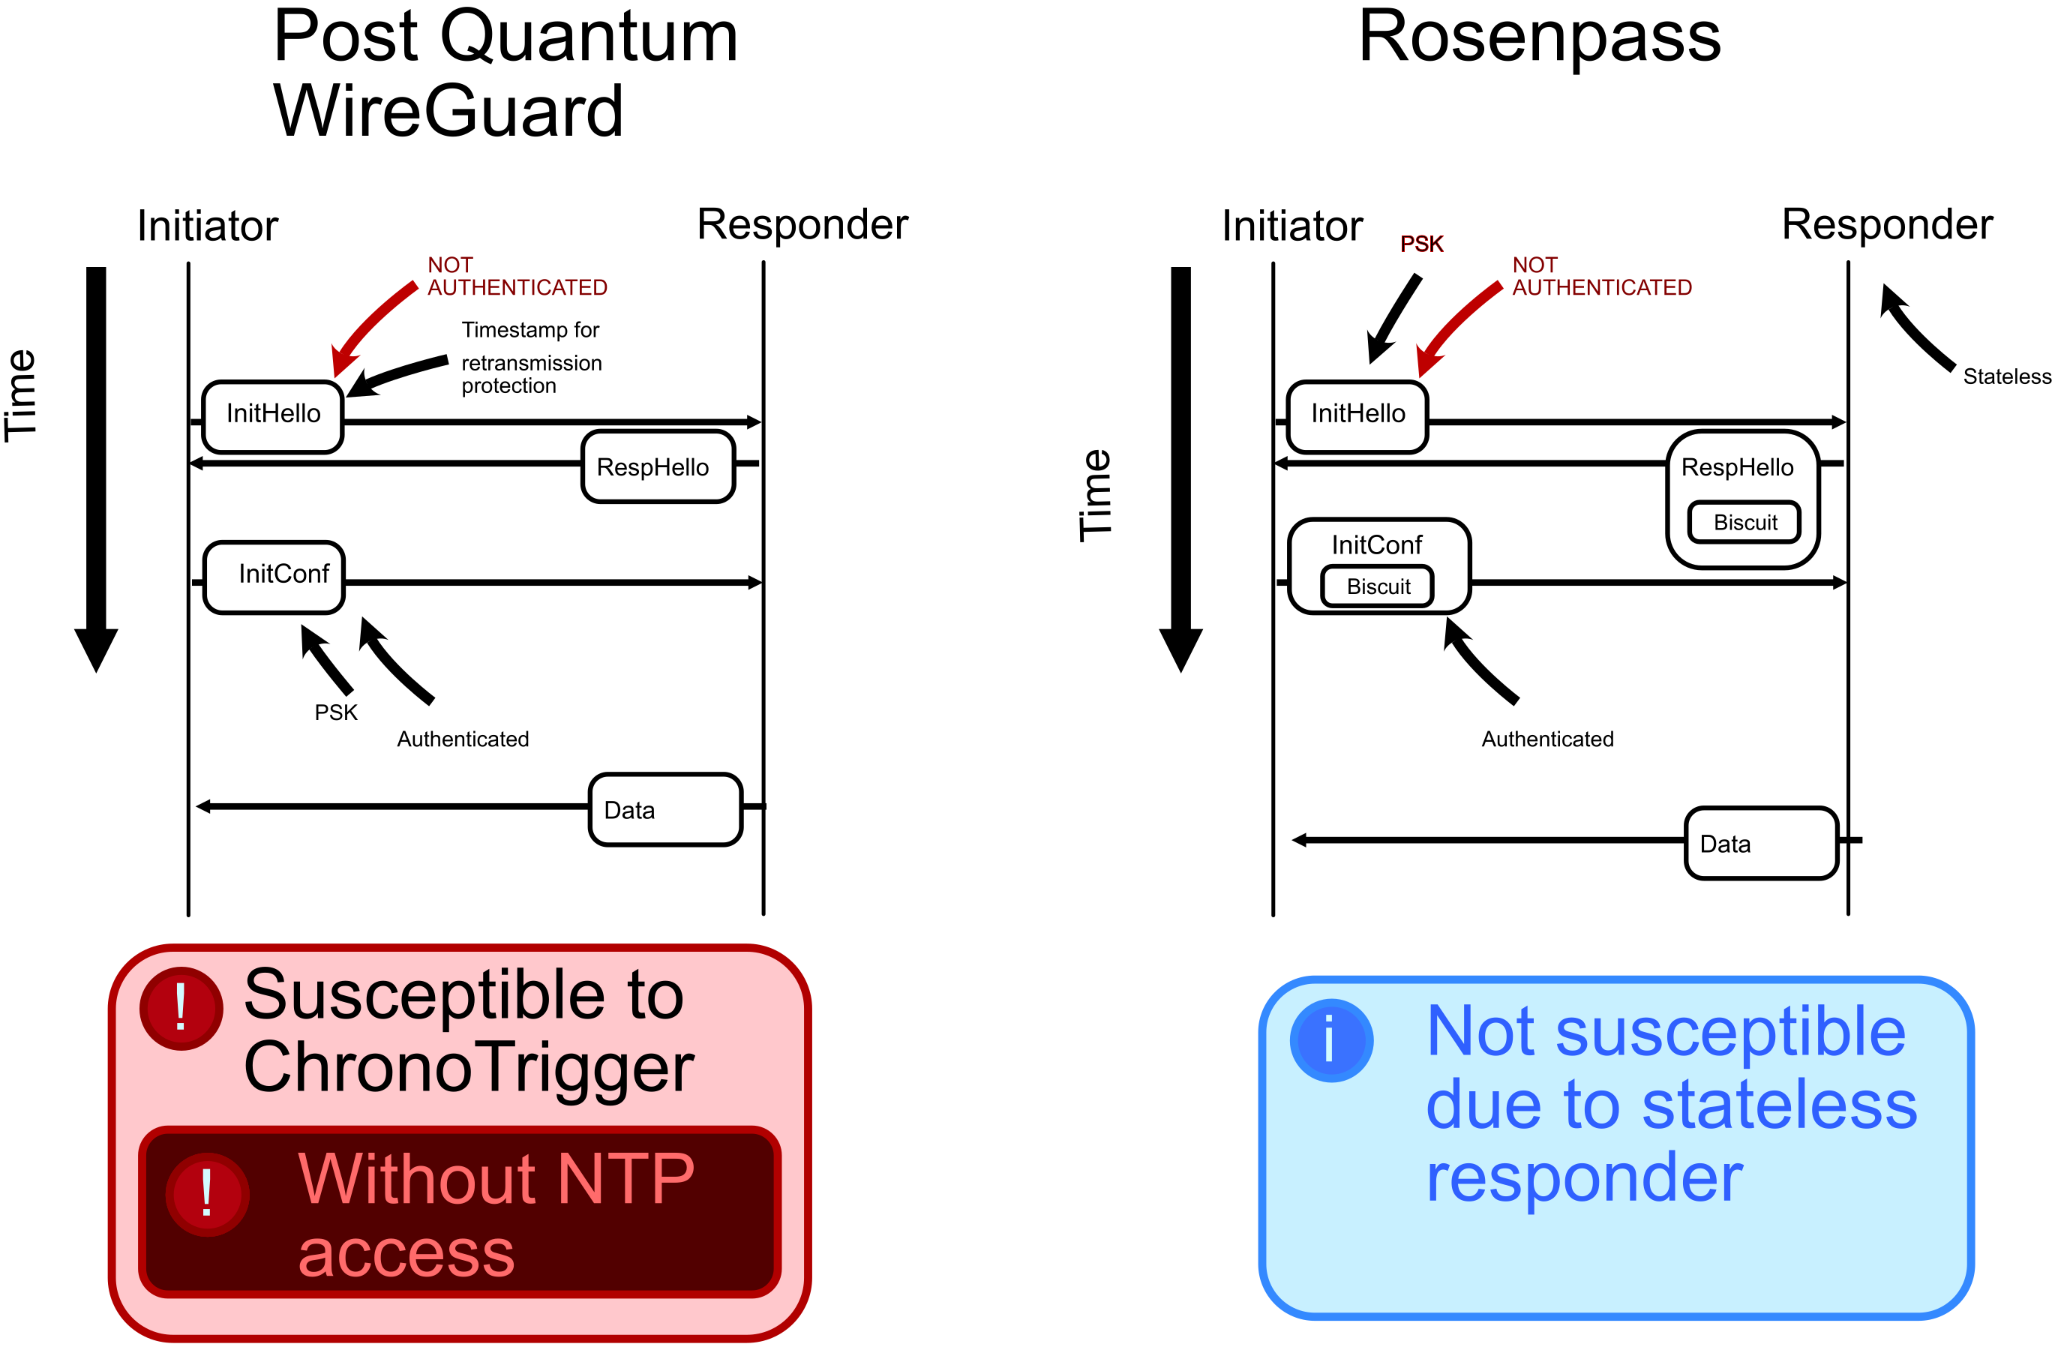
\includegraphics[keepaspectratio,width=.9\textwidth]{graphics/pqwg-rosenpass-compare.png}
      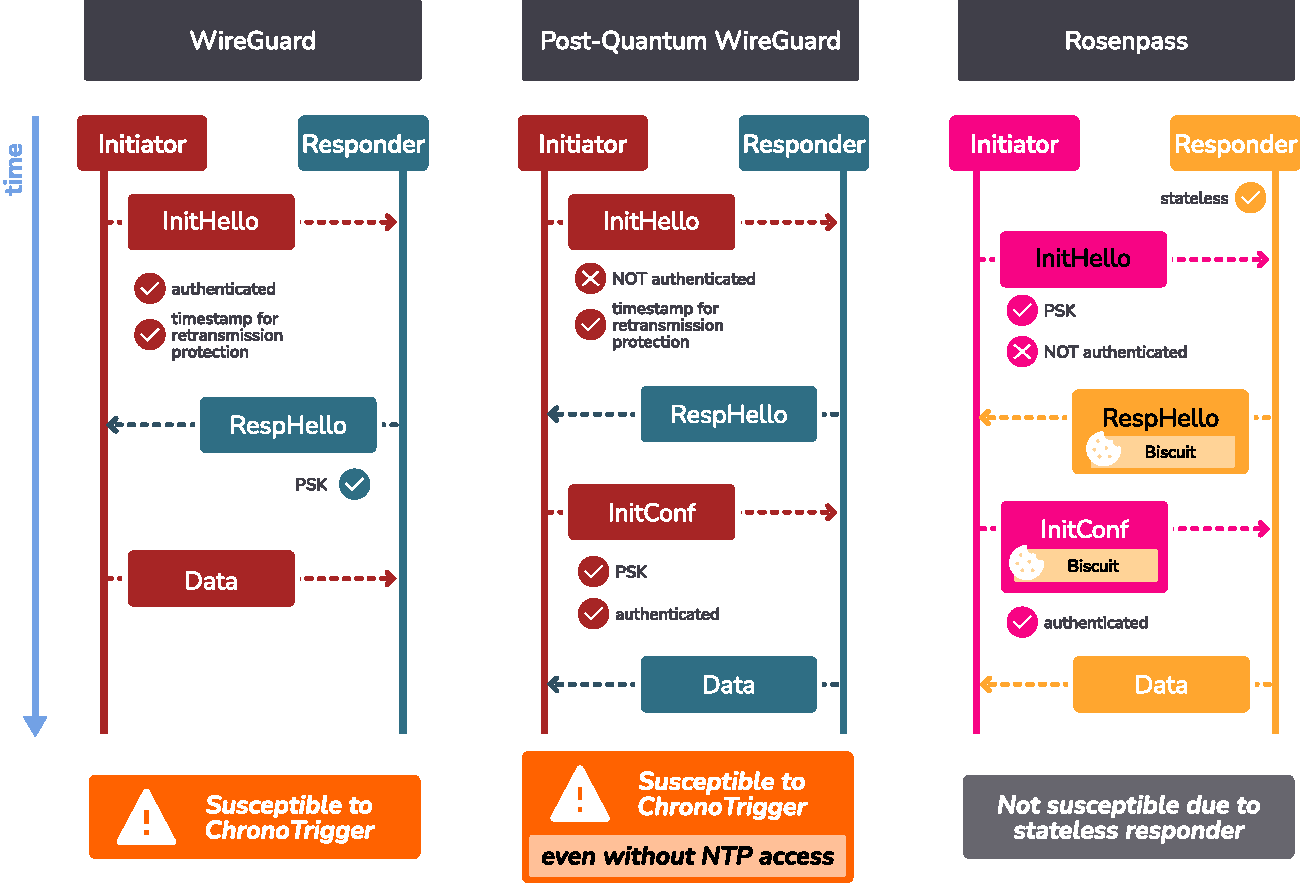
\includegraphics[keepaspectratio,width=\linewidth]{graphics/chronotrigger-compare.pdf}
    \end{column}%
    \begin{column}{.3\linewidth}
      \begin{itemize}
        \item InitHello remains unauthenticated
        \item PSK used in InitHello exclusively
        \item Responder state is moved into a cookie called \emph{Biscuit}
        \item[$\Rightarrow$] Stateless responder prevents ChronoTrigger attack
      \end{itemize}
    \end{column}
  \end{columns}
\end{frame}
